\chapter{Descobertas e sequências}
\markboth{Módulo 3}{}\enlargethispage{\baselineskip}

\section*{Habilidades do SAEB}

\begin{itemize}
\item Inferir ou descrever atributos ou propriedades comuns que os elementos
que constituem uma sequência recursiva de números naturais apresentam.

\item Inferir o padrão ou a regularidade de uma sequência de números
naturais ordenados, objetos ou figuras.

\item Inferir os elementos ausentes em uma sequência de números naturais
ordenados, objetos ou figuras.
\end{itemize}

\subsection{Habilidade da BNCC}

\begin{itemize}
\item EF03MA10.
\end{itemize}

\conteudo{
\begin{center}
\textbf{Sequências}
\end{center}

Uma sequência ou sucessão é um conjunto numérico ordenado, no qual existe sempre uma lógica de formação.

Na sequência numérica dos números naturais, com exceção do zero, todos os termos possuem um antecessor. O antecessor é o número imediatamente anterior na sequência. 

Na sequência numérica dos números naturais, todos os termos possuem um sucessor. O sucessor de um número é aquele imediatamente posterior na sequência. 

Exemplos de sequências

\begin{itemize}
\item 
  A escalação de um time de futebol de salão pode ser ordenada pela primeira letra dos nomes dos jogadores, ou seja, em ordem alfabética:
\end{itemize}

\begin{myquote}
\centering
\textbf{Alan, Bruno, Fernando, Igor, Tácio.}
\end{myquote}

\begin{itemize}
\item 
  Uma sequência pode ser formada pelos números pares:
\end{itemize}

\begin{myquote}
\centering
\textbf{0; 2; 4; 6; 8; 10; 12; ...}
\end{myquote}

As sequências podem ser classificadas quanto ao número de elementos que apresentam ou podem apresentar.

\begin{itemize}
\item
  Sequência finita apresenta número definido de termos,
  ou seja, 10 termos, 20 termos, 8 termos.
\item
  Sequência infinita apresenta número infinito de termos, como a sequência dos números naturais.
\end{itemize}

Ainda podemos classificar as sequências em:

\begin{itemize}
\item
  Sequência crescente: aquela em que cada termo sucessor é maior que seu antecessor.
\end{itemize}

\begin{myquote}
\centering
\textbf{Exemplo: 5, 10, 15, 20, 25.}
\end{myquote}

\begin{itemize}
\item
  Sequência decrescente: aquela em que cada termo sucessor sempre é menor do que seu antecessor.
\end{itemize}

\begin{myquote}
\centering
\textbf{Exemplo: 9, 7, 5, 3.}
\end{myquote}
}

\section*{Atividades}

\num{1} A professora Mariana colocou seus alunos posicionados em uma fila, 
%iniciada pelo aluno de tênis azul e mochila alaranjada, 
como na imagem a seguir.

\begin{figure}[htpb!]
\centering
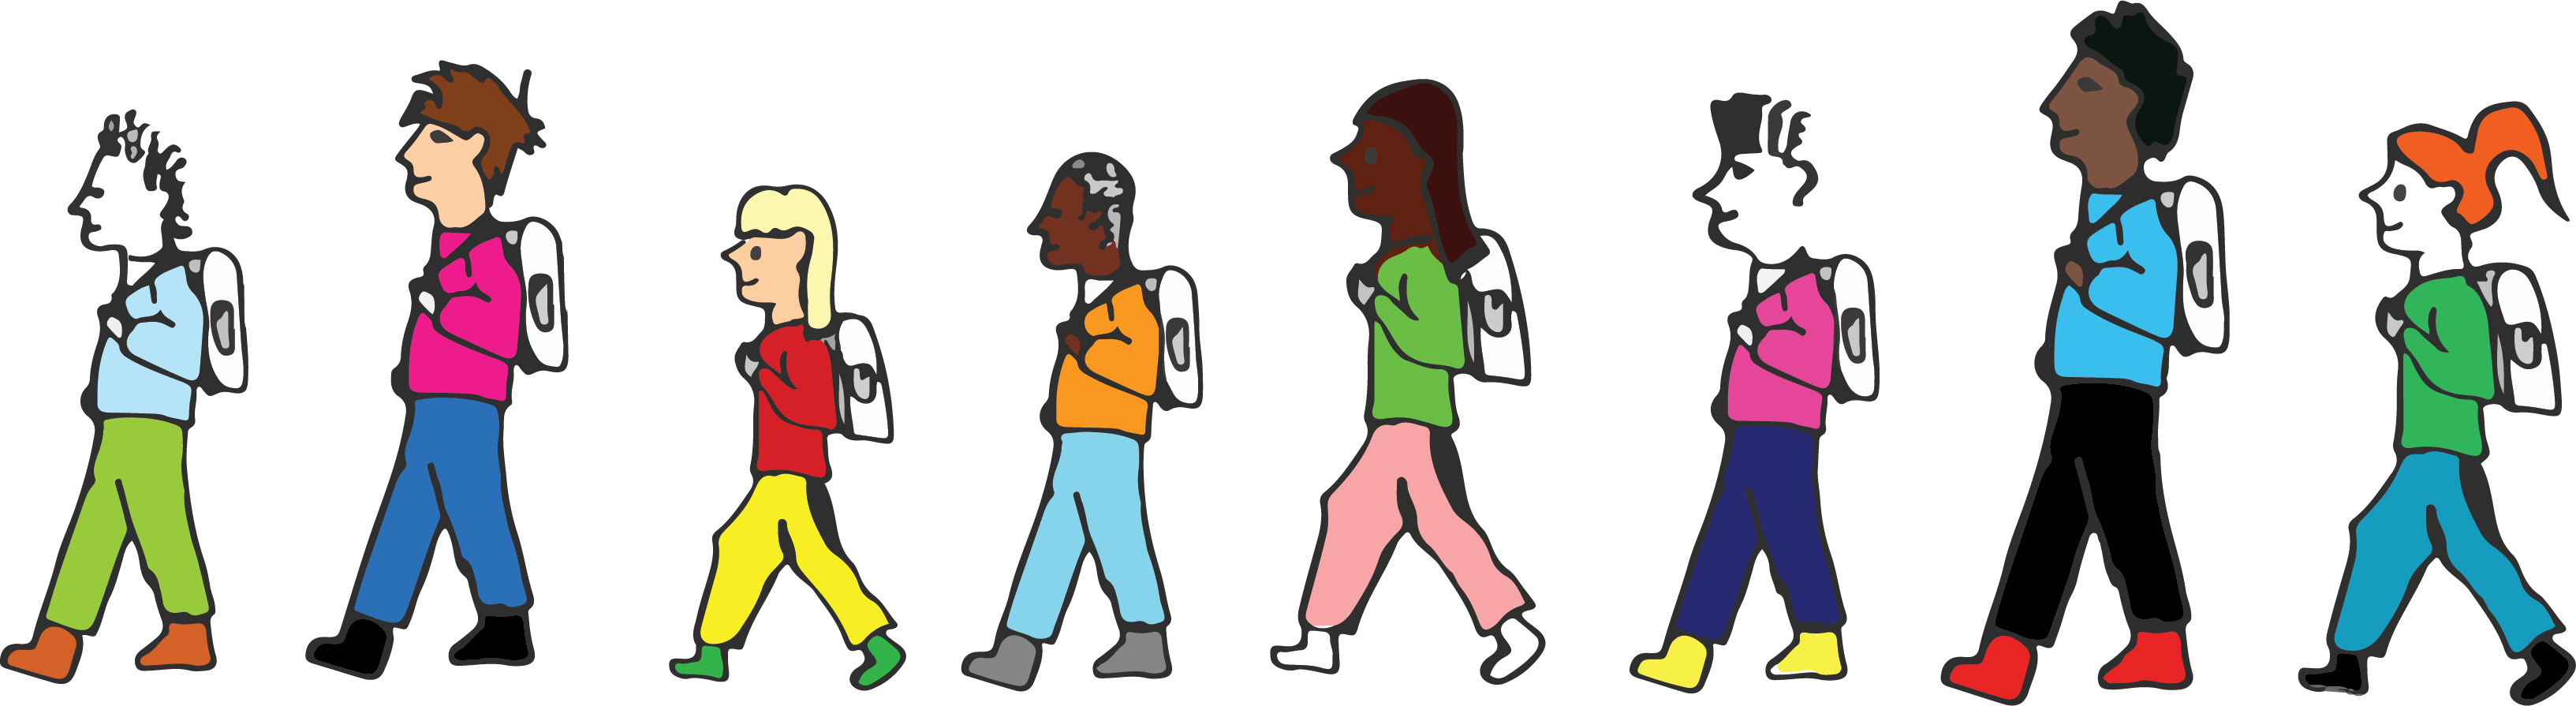
\includegraphics[width=\textwidth]{./media/image27.png}
\end{figure}

Observe atentamente a figura e responda ao que se pede.

\begin{escolha}
\item Qual a posição da criança mais baixa na fila? 
\reduline{A criança mais baixa está na 3º posição (terceira posição) na fila.\hfill}

\item Qual a posição da criança mais alta na fila? 
\reduline{A criança mais alta está na 7º posição (sétima posição) na fila.\hfill}
\end{escolha}

\num{2} O pai de Marcelo mostrou a ele uma sequência de bolinhas pintadas com
diversas cores.

\begin{figure}[htpb!]
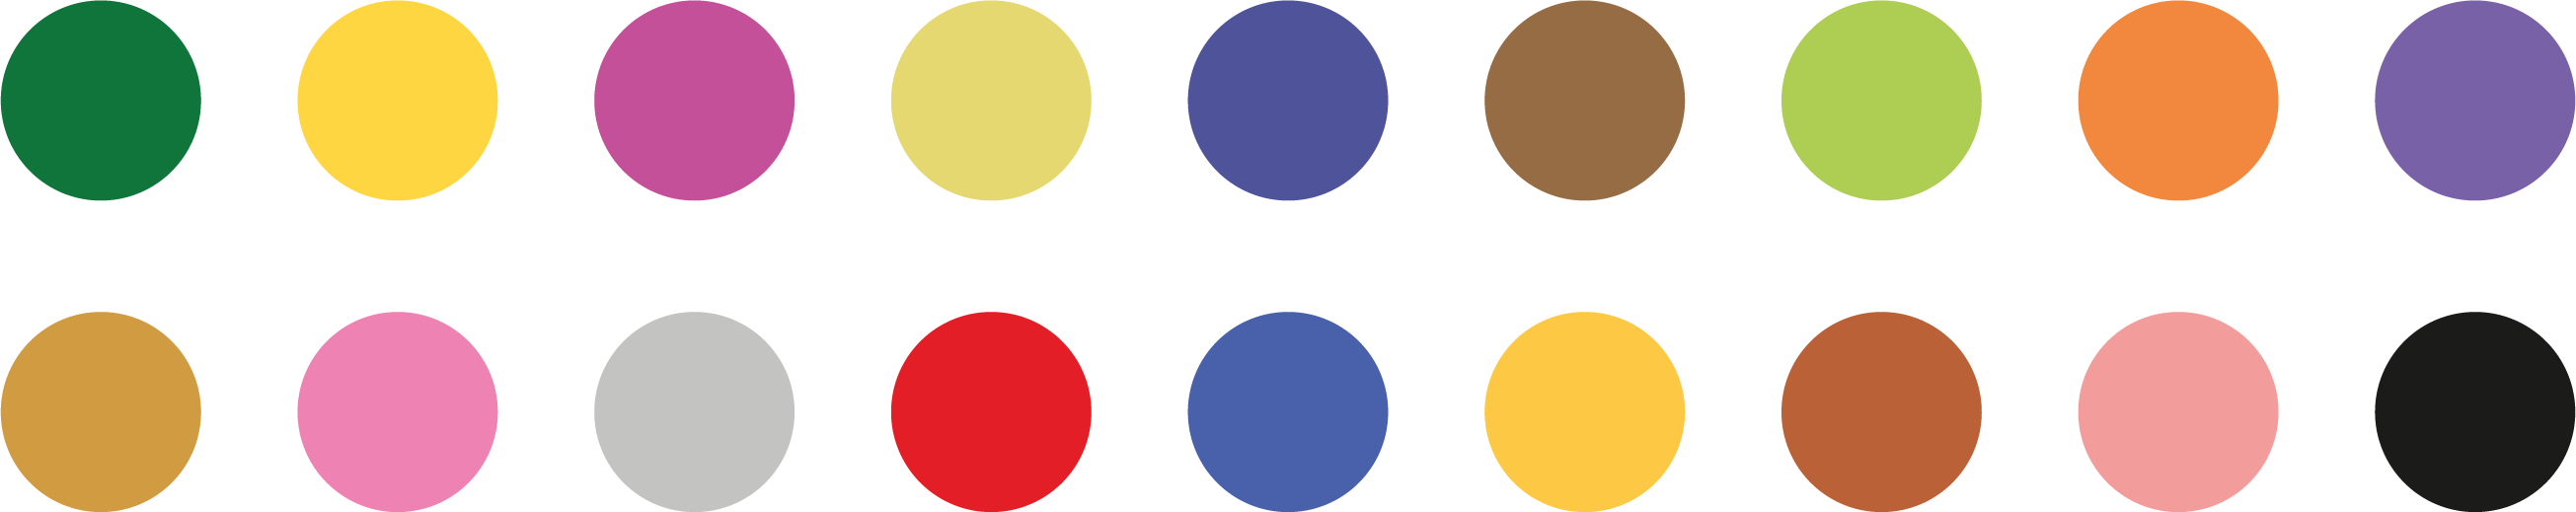
\includegraphics[width=\textwidth]{./media/image28.png}
\end{figure}

Observando essa sequência percebemos que a bolinha pintada com a cor
verde-escuro é a primeira, e a bolinha pintada com a cor preta é a
última.

Quais as posições das bolinhas pintadas com a cor azul?
\reduline{As bolinhas pintadas com a cor azul estão na 5º (quinta) posição e na
14º (décima quarta) posição.\hfill}


\num{3} Na prova de matemática que Manoela acabou de fazer estava o seguinte exercício:

\begin{myquote}
Escreva uma sequência de números de forma crescente, de 10 em 10, começando no número 705 até o sétimo termo.

%\begin{figure}[htpb!]
%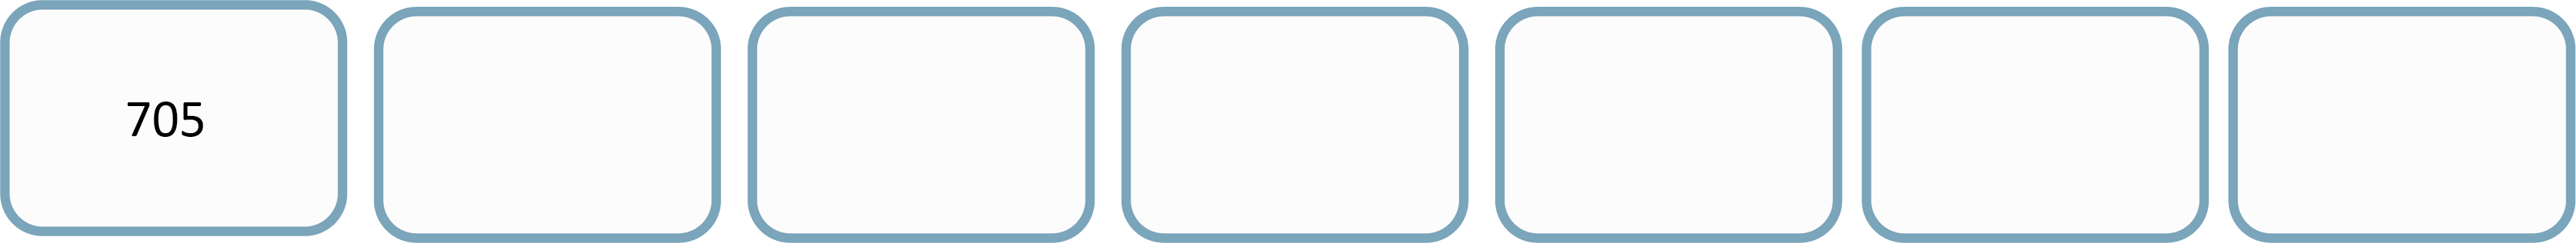
\includegraphics[width=\textwidth]{./media/image29.png}
%\end{figure}

\end{myquote}

Resolva a atividade proposta na prova de Manuela.
\reduline{705; 715; 725; 735; 745; 755; 765.\hfill}
\linhas{2}


\num{4} Rafaela foi a uma loja de brinquedos e, para ser atendida, pegou a senha de
número 32. Todos são atendidos pela ordem numérica das senhas.


%incluir imagem disponível em https://br.freepik.com/fotos-gratis/mulher-sorridente-segurando-o-cartao-de-visita-em-branco_24488868.htm#query=senha\%20de\%20atendimento\&position=41\&from_view=search\&track=robertav1_2_sidr

\begin{escolha}
\item Qual é o número da pessoa que foi atendida imediatamente antes de Rafaela?
\reduline{O número 31, pois é o antecessor de 32.\hfill}

\item Qual é o número da pessoa que será atendida imediatamente depois de Rafaela?
\reduline{O número 33, pois é o sucessor de 32.\hfill}
\end{escolha}

\pagebreak

\num{5} Alice organizou os nomes dos amigos que pretende convidar para sua
festa de aniversário em uma lista numerada.

\begin{figure}[htpb!]
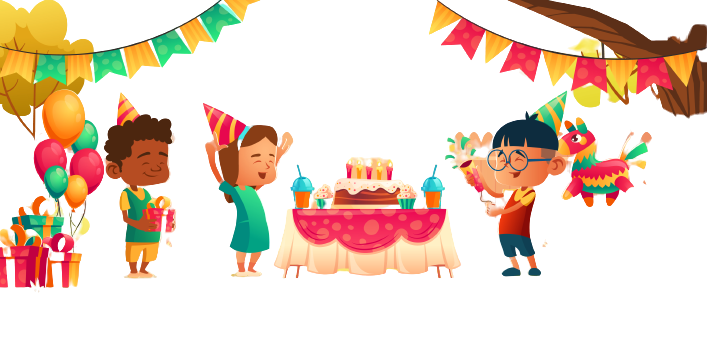
\includegraphics[width=\textwidth]{./media/image28a.png}
\end{figure}

\begin{myquote}
\begin{enumerate}
\begin{multicols}{2}
\item Ana

\item Ana Clara

\item Augusto

\item Bernardo

\item Camila

\item Daniel
\end{multicols}
\end{enumerate}
\end{myquote}

Observando a lista, responda ao que se pede.

\begin{escolha}
\item Qual o nome do amigo que aparece na posição do sucessor de 4?
\reduline{Camila, pois o sucessor do 4 é o 5.\hfill}

\item Qual o nome do amigo que aparece diante do antecessor de 3?
\reduline{Ana Clara, pois o antecessor do 3 é o 2.\hfill}

\item O número representado por Ana é antecessor de qual número?
\reduline{É antecessor de 2, já que Ana aparece no número 1.\hfill}
\end{escolha}

\pagebreak
\num{6} Observe o quadro que Roberta encontrou no caderno de seu irmão.

\begin{figure}[htpb!]
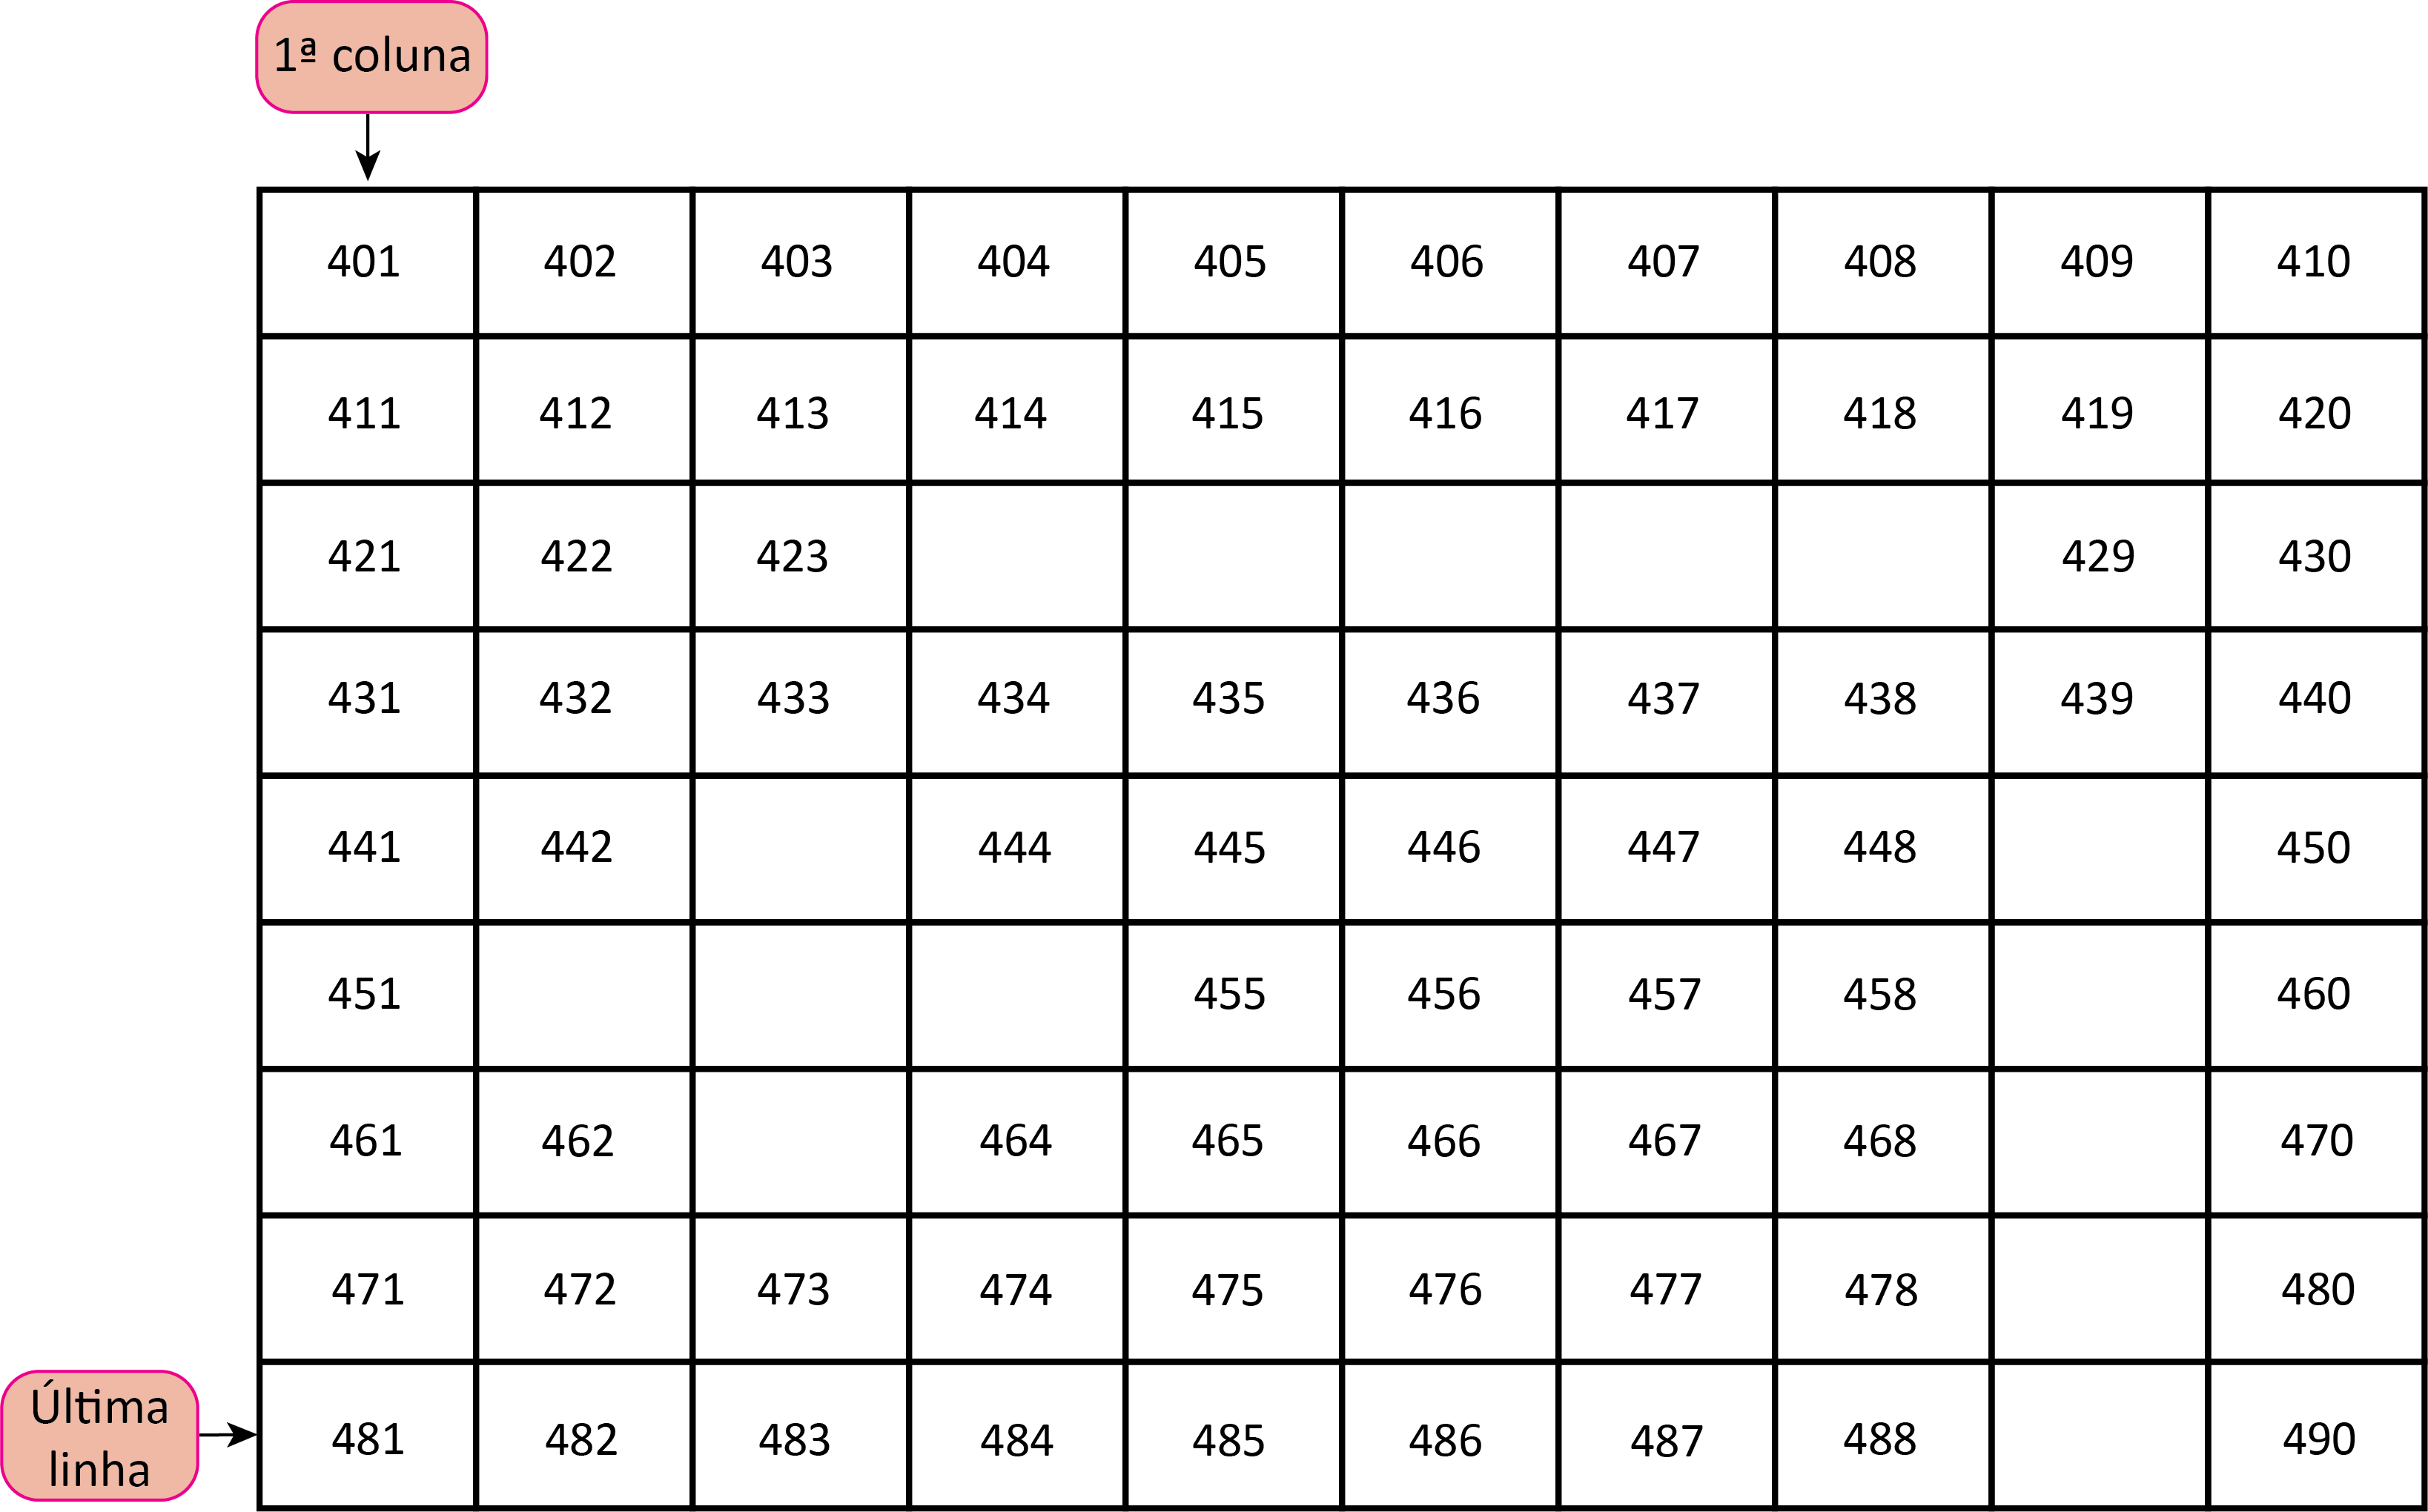
\includegraphics[width=\textwidth]{./media/image30.png}
\end{figure}

\begin{escolha}
\item Preencha os espaços vazios com os números que estão faltando.\coment{3ª linha: 424, 425, 426, 427, 428; 5ª linha: 443, 449; 6ª linha: 452, 453, 454, 459; 7ª linha: 463, 469; 8ª linha: 479; 9ª linha: 489.}

\item Qual é o número que está na 3ª coluna e na 4ª linha?
\reduline{433.\hfill}
\linhas{2}

\item Qual é a linha e a coluna em que o número quatrocentos e setenta e seis está?
\reduline{6ª coluna, 8ª linha.\hfill}
\linhas{2}
\end{escolha}

\vspace{-2ex}

\num{7} Observe a reta numérica que representa a sequência dos números naturais e responda a cada item a seguir.

\begin{figure}[htpb!]
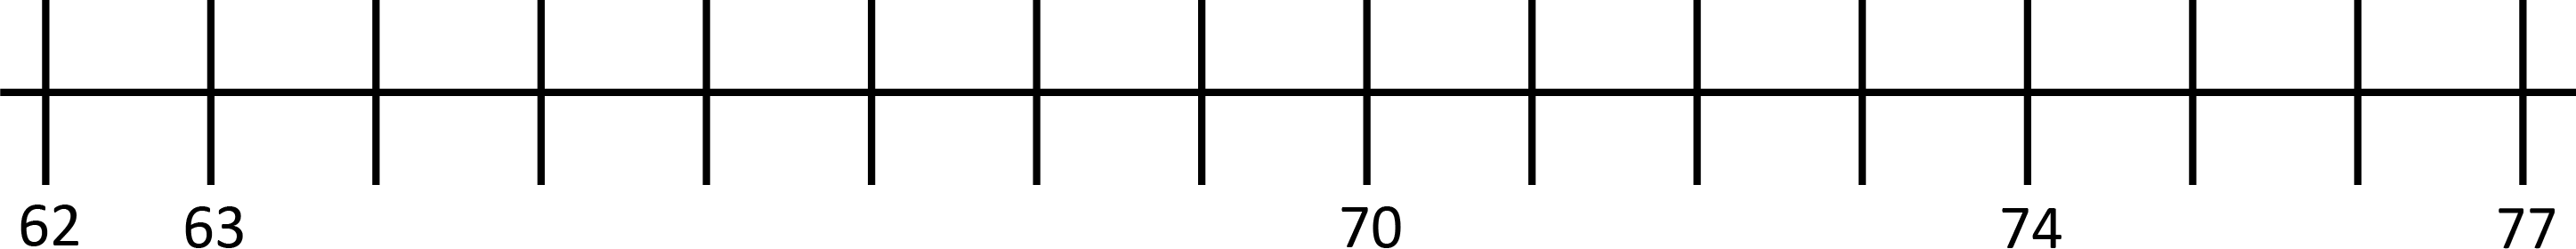
\includegraphics[width=\textwidth]{./media/image31.png}
\end{figure}

\begin{escolha}
\item Qual o número natural que será escrito imediatamente após o número 75?
\reduline{76, pois é o sucessor de 75.\hfill}

\item Qual o número natural que virá escrito antes do número 68 nessa reta numérica?
\reduline{67, pois é o antecessor de 68.\hfill}

\item Qual o antecessor do número setenta e sete?
\reduline{76.\hfill}

\item Qual o sucessor do número setenta e quatro?
\reduline{75.\hfill}
\end{escolha}

\num{8} Escreva os números naturais de cada item em ordem crescente.

\begin{escolha}
\item 30; 25; 10; 5; 20; 15
\reduline{5; 10; 15; 20; 25; 30.\hfill}

\item 7; 21; 14; 35; 28
\reduline{7; 14; 21; 28; 35.\hfill}

\item 16; 8; 12; 4; 24; 20
\reduline{4; 8; 12; 16; 20; 24.\hfill}
\end{escolha}

\num{9} Em cada item, indique se a sequência é crescente ou decrescente.

\begin{escolha}
\item 10; 8; 6; 4; 2; 0
\reduline{Decrescente.\hfill}

\item 10; 20; 30; 40; 50
\reduline{Crescente.\hfill}

\item 21; 19; 17; 15; 13
\reduline{Decrescente.\hfill}

%\item 6; 12; 18; 24; 30; 36
%\reduline{Crescente.\hfill}
\end{escolha}

\num{10} Observe as sequências dadas e determine, sem fazer desenhos, a
quantidade de bolinhas que a figura 8 de cada sequência terá.

\begin{escolha}
\item \reduline{3; 6; 9; 12; 15; 18; 21; 24; ou 3 x 8 = 24.\hfill} bolinhas

\begin{center}
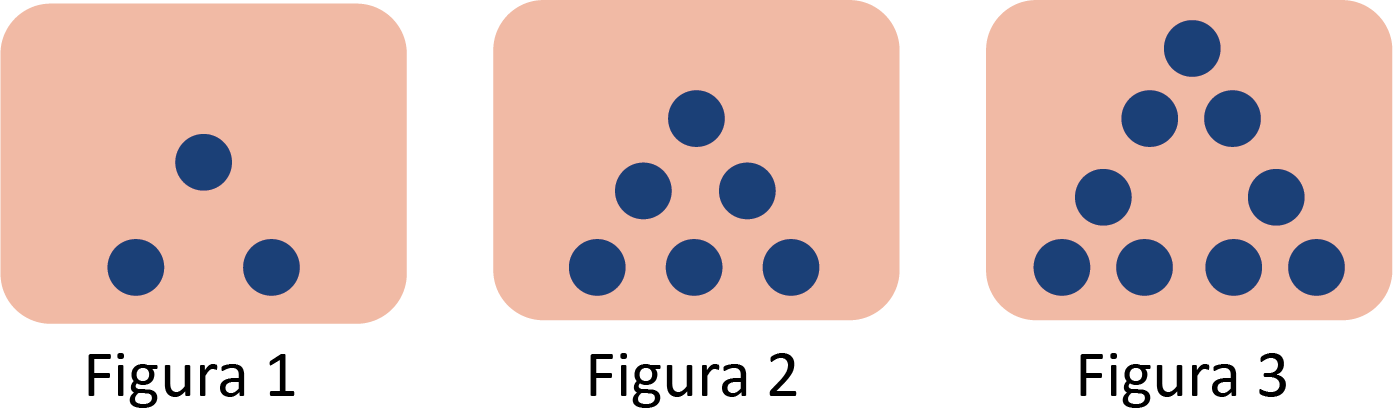
\includegraphics[width=.7\textwidth]{./media/image33.png}
\end{center}

\item \reduline{4; 8; 12; 16; 20; 24; 28; 32; ou 8 x 4 = 24.\hfill} bolinhas

\begin{center}
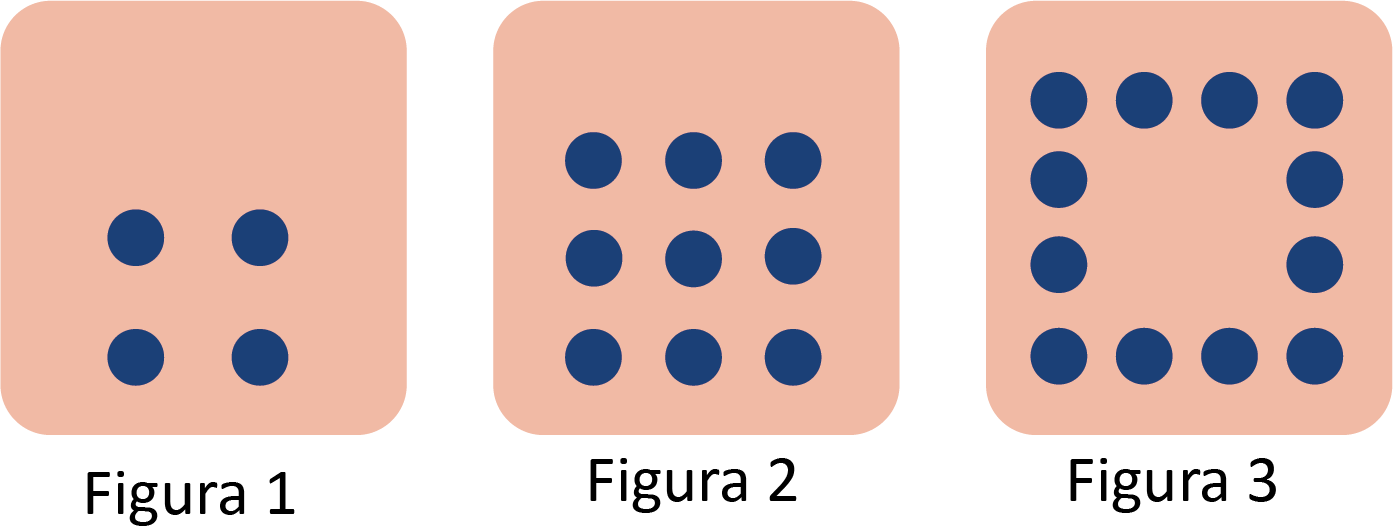
\includegraphics[width=.7\textwidth]{./media/image34.png}
\end{center}
\item \reduline{5; 10; 15; 20; 25; 30; 35 40; ou 5 x 8 = 40.\hfill} bolinhas

\begin{center}

\includegraphics[width=.7\textwidth]{./media/image35.png}
\end{center}
\end{escolha}

\pagebreak

\num{11} Encontre o número pedido em cada item.

\begin{escolha}
\item O sucessor de 4.089 \reduline{4.090\hfill}

\item O antecessor de 4.302 \reduline{4.301\hfill}

\item O sucessor e o antecessor do número 5.259 \reduline{5.258 e 5.260.\hfill}
\end{escolha}

%\coment{Vale explorar bastante os conceitos de sucessor e antecessor com os alunos, pois isso facilitará muitos entendimentos em anos futuros.}

\num{12} Ana Clara encontrou um papel entre os cadernos de seu irmão mais velho, com as seguintes anotações:

\begin{myquote}
\centering
\textbf{(21; 58; 95; 132; ...)}
\end{myquote}

Ela ficou muito curiosa, pois entendeu que essa era uma sequência
numérica e queria encontrar o próximo número dessa sequência.

Ajude Ana Clara a descobrir qual é o próximo número da sequência e escreva-o no espaço disponível.

\reduline{A sequência foi montada sempre somando 37 ao número anterior para
encontrar o próximo. Portanto, o próximo número da sequência será: 132 + 37 = 169.\hfill}
\linhas{3}

\begin{comment}
\num{13} A professora de Camila decidiu propor um desafio à turma. Assim, apresentou uma sequência de figuras e pediu que os alunos descobrissem qual seria a próxima imagem. 

%Usar recortes da imagem disponível em https://br.freepik.com/vetores-gratis/cartoes-de-jogo-de-memoria-desenhados-a-mao_37451777.htm#query=sequ%C3%AAncias%20de%20figuras&position=0&from_view=search&track=robertav1_2_sidr  
%para construir a seguinte sequência:bola-quadrado-quadrado-losango-triângulo-triângulo-triângulo-oval-bola-quadrado-quadrado-losango-triângulo

Quem acertou o desafio foi o colega de Camila, Gabriel. Qual foi a resposta dele?

\reduline{Gabriel respondeu que a próxima figura seria um triângulo.\hfill}

\reduline{É possível que o aluno continue a sequência com desenhos até chegar à resposta. Não há problemas na utilização dessa técnica.\hfill}
\linhas{1}
\end{comment}

\num{13} Observe as sequências e complete-as com os números que estão faltando.

\begin{escolha}
\item 102 \quad \reduline{104}\quad 106 \quad \reduline{108} 110 \quad \reduline{112}

\item 85 \quad \reduline{90} \quad \reduline{95} \quad 100 \quad 105 \quad \reduline{110}
\end{escolha}


\pagebreak

\section*{Treino}

\num{1} Se os números escritos a seguir foram colocados em ordem crescente, qual
é o número que fica imediatamente antes de 63?

\begin{myquote}
\centering
\textbf{95; 63; 25; 76; 54; 68; 48.}
\end{myquote}

\begin{escolha}
\begin{multicols}{2}
% Conteúdo da primeira coluna
\item 25.

\item 48.
\end{multicols}

% Conteúdo entre as duas colunas

\begin{multicols}{2}
% Conteúdo da segunda coluna
\item 54.

\item 68.
\end{multicols}
\end{escolha}

\num{2} Observe a sequência e marque a alternativa que corresponde ao número de bolinhas que a figura 6 terá.

\vspace{1em}
%\begin{figure}[htpb!]
%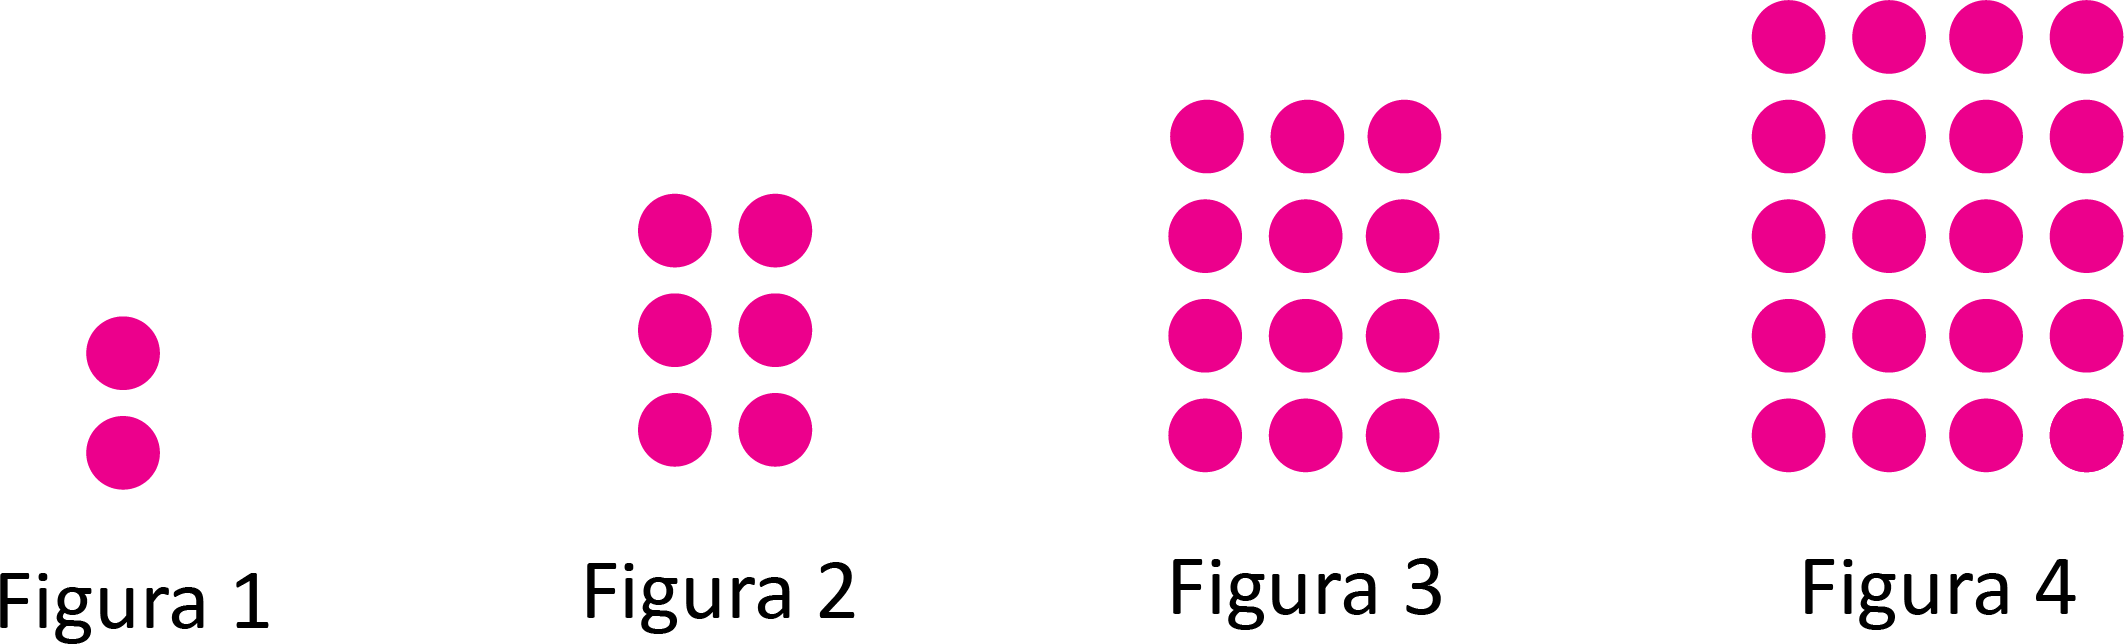
\includegraphics[width=\textwidth]{./media/image37.png}
%\end{figure}

%\item \reduline{4; 7; 10; 13; 16; 19; 22; 25; ou (8 x 3) + 1 = 25.\hfill} bolinhas

\begin{center}
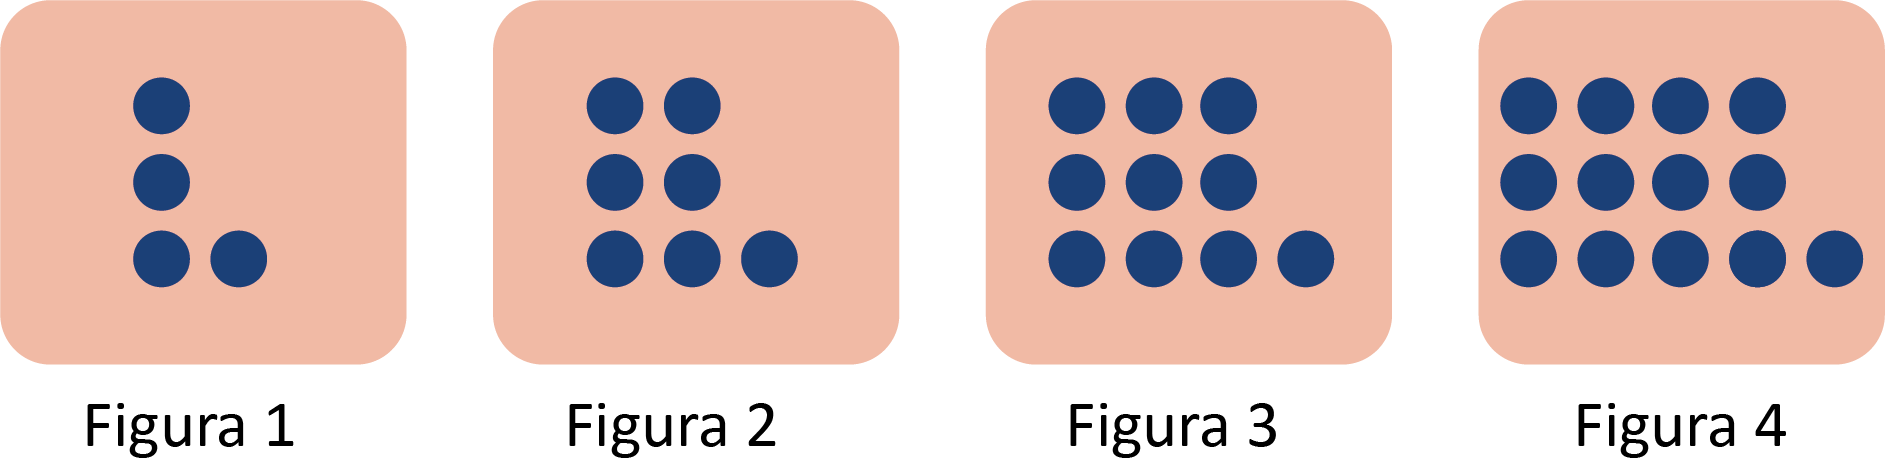
\includegraphics[width=.7\textwidth]{./media/image32.png}
\end{center}

\begin{escolha}

\begin{multicols}{2}
% Conteúdo da primeira coluna

\item 9.

\item 16.
\end{multicols}

% Conteúdo entre as duas colunas

\begin{multicols}{2}
% Conteúdo da segunda coluna

\item 12.

\item 19.
\end{multicols}
\end{escolha}

\num{3} Assinale a alternativa que possui uma sequência que traz um antecessor, um número e seu sucessor.

\begin{escolha}
\item 450; 455; 460.

\item 526; 626; 726.

\item 436; 446; 456.

\item 488; 489; 490.
\end{escolha}

